\chapter{Vacuum Energy, Expansion, and de Sitter Horizons}

These notes follow Leonard Susskind's eighth lecture in the supplementary \emph{Cosmology and Black Holes} track, keeping close to the order in which the lecture actually develops. The lecture begins not with a formal derivation but with student questions: what vacuum energy is, why it does not behave like an ordinary medium, why it matters gravitationally, and only then how it leads to accelerated expansion and event horizons. The aim here is to preserve that narrated progression while writing the mathematics in a clean form. These notes are presented as a companion to Leonard Susskind's lecture and are curated by LazyingArt LLC.

\section{Vacuum Energy, Virtual Fluctuations, and Lorentz Invariance}

The first question in the lecture is operational: if virtual electron--positron pairs contribute to the vacuum energy, does that mean that particles should literally pop out of empty space? Susskind's answer is no. The vacuum is not a state in which ordinary particles are being produced in the observable sense. Rather, it is the quantum ground state, and the right analogy is the harmonic oscillator. Classically the oscillator can sit motionless at the bottom of its potential, but quantum mechanically the ground state still carries energy,
\begin{equation}
E_{\rm zp}=\frac{1}{2}\hbar\omega.
\end{equation}
That is the first mathematical entry point into the lecture's discussion. The electromagnetic field in a cavity may be viewed as a collection of oscillators; each contributes zero-point energy, and the collection contributes to what the lecture calls the vacuum energy.

The second question is the more revealing one. If empty space contains positive energy density, why does it not act like a material medium and change the local speed of light? Susskind answers this by distinguishing ordinary matter from vacuum energy. Ordinary matter picks out a preferred rest frame. A gas, for example, looks different to an observer moving rapidly through it than to one moving with it. Vacuum energy is special precisely because it does not do that. If one imagines a ``vacuum-energy detector,'' the reading is the same for every inertial observer. In that sense the presence of vacuum energy does not define a preferred Lorentz frame.

This is the real conceptual pivot of the lecture. Vacuum energy is not merely some extra stuff hidden in space. It is the one form of energy density that preserves the Lorentz-invariant character of empty space. In the notation used later in the lecture, one writes
\begin{equation}
\rho_{\rm vac}=\text{const.}
\end{equation}
The point here is not yet the cosmological time dependence, but the fact that vacuum energy does not change when the observer changes velocity. Susskind immediately links this to the local statement that light, when it passes right by a local observer with local clocks and rulers, is still measured to move with speed \(c\). Only later does he return to the subtler question of how light behaves relative to us when it is very far away in an expanding universe.

\section{Why Gravity Forces the Issue}

The lecture now makes a sharp transition. In ordinary laboratory physics one usually cares only about \emph{differences} of energy. The absolute zero of energy can often be shifted without consequence. Susskind stresses that this changes once gravity enters. Gravity couples to energy itself. If vacuum energy exists, then it gravitates; it affects the geometry of spacetime.

At this stage he pauses to remind the audience of the structure of Einstein's equations. The geometric side is built from the metric tensor \(g_{\mu\nu}(x)\), and the material side is built from the energy and momentum of matter and fields. For the purposes of this lecture, the only point that matters is the division into geometry and source, so it is enough to write schematically
\begin{equation}
G_{\mu\nu}\propto T_{\mu\nu}.
\end{equation}
The proportionality constant is not the issue here. The lecture only needs the reader to remember that geometry sits on the left and energy-momentum on the right.

\begin{figure}[htbp]
\centering

\includegraphics[width=0.58\textwidth]{lecture_08_figure_02.png}
\caption{Documentary board state at the moment Susskind identifies \(G_{\mu\nu}\) as the geometric side of Einstein's equations and writes the underlying metric notation \(g_{\mu\nu}(x)\).}
\end{figure}

The lecture then narrows immediately to a very special geometry: spatially flat space expanding uniformly in time. In the blackboard notation preserved in the lecture frames, the metric is written as
\begin{equation}
ds^2=-dt^2+a(t)^2\,dx^2.
\end{equation}
Here \(dx^2\) is shorthand for the Euclidean spatial line element \(dx^2+dy^2+dz^2\). The new ingredient is the scale factor \(a(t)\), a function of time only. It tells us that the coordinate labels on space stay fixed while the physical distance between coordinate marks changes with time. If two points have fixed coordinate separation \(\Delta x\), their physical separation is
\begin{equation}
D_{\rm phys}(t)=a(t)\,\Delta x.
\end{equation}
This is exactly the ``rubber sheet'' picture used in the lecture. Once the geometry is reduced to this ansatz, Einstein's equations become equations for the time dependence of \(a(t)\).

\section{The Friedmann Equation and the Matter-Dominated Branch}

For the spatially flat metric above, the lecture writes the cosmological field equation in the form
\begin{equation}
\left(\frac{\dot a}{a}\right)^2=\frac{8\pi G}{3}\rho(t),
\end{equation}
where \(\rho(t)\) is the homogeneous energy density filling the universe.

\begin{figure}[htbp]
\centering

\includegraphics[width=0.86\textwidth]{lecture_08_figure_04.png}
\caption{The clearest surviving board frame for the metric \(ds^2=-dt^2+a(t)^2dx^2\) and the corresponding Friedmann equation \(\left(\dot a/a\right)^2=(8\pi G/3)\rho(t)\).}
\end{figure}

At this point the lecture does not rush to a solution. It first asks a more physical question: what does \(\rho(t)\) do for ordinary matter? Susskind answers by returning to a box argument. Take a comoving box whose coordinate side length is \(\Delta x\). Its physical side length is \(a(t)\Delta x\), so its physical volume is \(a(t)^3(\Delta x)^3\). If that box contains \(n\) nonrelativistic particles of mass \(m\), then
\begin{equation}
\rho_m(t)=\frac{nm}{a(t)^3(\Delta x)^3}.
\end{equation}
In the lecture he chooses the mathematical box so that \(\Delta x=1\), and then the point is transparent:
\begin{equation}
\rho_m(t)=\rho_0\,a(t)^{-3}.
\end{equation}
Ordinary matter dilutes because the number of particles and their masses stay fixed while the volume grows.

Now the equation for \(a(t)\) closes:
\begin{equation}
\left(\frac{\dot a}{a}\right)^2=\frac{8\pi G}{3}\frac{\rho_0}{a^3}.
\end{equation}
This is the moment in the lecture where Susskind says, in effect, ``maybe we should solve it.'' The solution is elementary but worth working through because the physical conclusion depends on the algebra.

\paragraph{Worked derivation.}
Absorb the constant \((8\pi G/3)\rho_0\) into a single positive constant \(K\). Then
\begin{align}
\left(\frac{\dot a}{a}\right)^2&=K a^{-3},\\
\dot a^2&=K a^{-1}.
\end{align}
Taking the expanding branch,
\begin{equation}
\dot a=\sqrt{K}\,a^{-1/2}.
\end{equation}
Separate variables:
\begin{equation}
a^{1/2}\,da=\sqrt{K}\,dt.
\end{equation}
Integrating gives
\begin{equation}
\frac{2}{3}a^{3/2}=\sqrt{K}\,t+\text{constant}.
\end{equation}
Ignoring inessential normalization constants,
\begin{equation}
a(t)\propto t^{2/3}.
\end{equation}

This is the matter-dominated cosmology developed in the lecture. It is not linear expansion. The graph bends over: the universe decelerates. Susskind's physical reading is that matter makes gravity important, and gravity slows the original outward motion down.

He then inserts one brief comparison that is important for orientation but not pursued in detail. If the universe were dominated by radiation rather than nonrelativistic matter, the density would behave as
\begin{equation}
\rho_{\rm rad}(t)\propto a(t)^{-4}.
\end{equation}
That contrast is mentioned only to sharpen the new point: vacuum energy will be different from both matter and radiation.

\paragraph{The lecture's heuristic energy-conservation reading.}
Before leaving the matter-dominated branch, Susskind pauses over a reformulation that he explicitly calls an ``energy conservation'' reading of the equation. He treats the matter term as positive and the time-dependent gravitational piece as negative, so that the Friedmann equation can be read heuristically as
\begin{equation}
-\left(\frac{\dot a}{a}\right)^2+\frac{8\pi G}{3}\rho(t)=0.
\end{equation}
The point is not the exact coefficient of the gravitational contribution; the point is the sign. In the lecture, the time dependence of the geometry carries a negative contribution, and ``minus this plus this equals zero'' is the mnemonic form.

\begin{remark}
This is a faithful representation of the lecture, but it should remain a lecture-specific heuristic for this minisuperspace cosmology. It is not a general claim that one has a globally conserved total energy in an arbitrary expanding spacetime.
\end{remark}

\begin{figure}[htbp]
\centering

\includegraphics[width=0.82\textwidth]{lecture_08_figure_03.png}
\caption{Intermediate board state from the lecture. The left edges are cropped, so the notes typeset the metric and Friedmann equation in their standard forms nearby, while the screenshot preserves the in-progress two-line board layout that Susskind then interprets heuristically as an energy-balance equation.}
\end{figure}

\section{Vacuum Energy and Exponential Expansion}

Only after the matter-dominated case is in hand does the lecture pivot to the new ingredient. Vacuum energy does not dilute. In the lecture's preferred notation,
\begin{equation}
\rho(t)=\rho_{\rm vac}=\text{const.}
\end{equation}
One could equivalently introduce a cosmological constant \(\Lambda\) after a trivial rescaling, but the lecture itself mostly speaks in terms of the density \(\rho_{\rm vac}\), and it is better to keep that language here.

Substituting a constant density into the Friedmann equation gives
\begin{equation}
\left(\frac{\dot a}{a}\right)^2=\frac{8\pi G}{3}\rho_{\rm vac}.
\end{equation}
Because the right-hand side is now constant, Susskind names it \(H^2\):
\begin{equation}
H^2=\frac{8\pi G}{3}\rho_{\rm vac}.
\end{equation}
At this stage \(H\) is more than the formal definition \(\dot a/a\); it is also a constant number determined by the vacuum energy density. The evolution equation becomes
\begin{equation}
\dot a=Ha,
\end{equation}
and this is the place where the lecture's spoken line gets garbled. The clean mathematical statement is simply
\begin{equation}
a(t)=C e^{Ht},
\end{equation}
with \(C\) an integration constant.

This is the second great cosmological branch of the lecture. In the matter-dominated case the universe decelerates. In the vacuum-dominated case the growth rate is proportional to the size itself, and the expansion is exponential. Susskind then immediately translates this into the Hubble-law language used observationally:
\begin{equation}
v=HD.
\end{equation}
If \(H\) is constant, then the distance at which recession speed reaches the speed of light is
\begin{equation}
D_H=\frac{c}{H}.
\end{equation}
The lecture uses this as the first sign that the pure vacuum geometry comes with a fixed characteristic distance scale.

Susskind does not stop with the pure case. He immediately returns to the real universe, where matter and vacuum energy coexist. Early on, when \(a\) is small, the diluting matter term \(a^{-3}\) dominates; later, as \(a\) grows, that term shrinks while \(\rho_{\rm vac}\) stays fixed. Therefore the lecture's qualitative history is
\begin{equation}
a(t)\sim t^{2/3}\qquad\text{at early times},
\end{equation}
followed by
\begin{equation}
a(t)\sim e^{Ht}\qquad\text{at late times}.
\end{equation}
This is the point at which Susskind turns from theory to observation. He says that one can check whether \(H\) stays constant, or equivalently whether the late-time scale factor is well fit by an exponential, by looking out into the distant universe and thereby looking back in time. The lecture's claim is that the data look convincingly like the late-time exponential branch.

\begin{figure}[htbp]
\centering
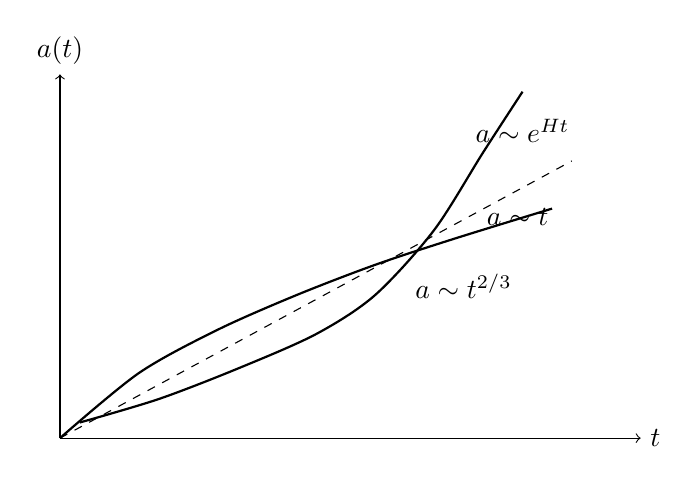
\begin{tikzpicture}[x=1.25cm,y=1.1cm]
\draw[->] (0,0) -- (5.9,0) node[right] {$t$};
\draw[->] (0,0) -- (0,4.2) node[above] {$a(t)$};

\draw[dashed] (0,0) -- (5.2,3.2);
\node at (4.65,2.55) {$a\sim t$};

\draw[thick] plot[smooth] coordinates {(0,0) (0.8,0.75) (1.6,1.25) (2.4,1.65) (3.2,2.0) (4.0,2.3) (5.0,2.65)};
\node at (4.1,1.75) {$a\sim t^{2/3}$};

\draw[thick] plot[smooth] coordinates {(0.2,0.18) (1.0,0.45) (1.8,0.8) (2.6,1.2) (3.2,1.65) (3.8,2.4) (4.3,3.3) (4.7,4.0)};
\node at (4.7,3.55) {$a\sim e^{Ht}$};
\end{tikzpicture}
\caption{Transcript-backed reconstruction of the lecture's qualitative comparison between linear growth, the matter-dominated law \(a\sim t^{2/3}\), and the late-time exponential takeoff driven by vacuum energy.}
\end{figure}

\section{Bound Systems, Escape, and the Observational Future}

Before the lecture reaches de Sitter geometry, it cashes out the physical meaning of exponential expansion in a more conversational way. If vacuum energy dominates forever, then all matter and radiation that dilute with expansion become more and more negligible. The remaining question is whether local bound structures are also dragged apart.

Susskind's answer is no. The key distinction is not ``does gravity exist here?'' but ``is the system gravitationally bound?'' That is why he immediately discusses nearby galaxies. Andromeda is not simply another distant object in the Hubble flow. Its relative motion to us is a local accident of the nearby gravitational environment, and the lecture treats it as part of the small set of objects that will not simply drift away. Distant galaxies that are not bound behave differently: they continue with the flow and eventually disappear from view.

The lecture becomes especially careful here because the audience pushes on the phrase ``gravitationally bound.'' Susskind distinguishes two different claims. One claim is dynamical dominance: at a given distance, ordinary gravity may be the largest force. The other claim is binding: whether an object will in fact remain attached rather than escape. These are not the same statement. His rocket analogy makes the point clearly: a rocket fired above escape velocity is not bound to Earth even though Earth's gravity is still the dominant force acting on it for a long part of its trajectory.

He also allows himself a Newtonian picture, but only as an intuition. One may think of an attractive term that falls like \(1/r^2\) together with a very weak outward effect associated with vacuum energy that grows with distance. The lecture does not fix the coefficient of that outward term, and it is better not to overstate it here. The point is qualitative: the vacuum contribution is tiny on laboratory scales, modest even on galactic scales, and only becomes competitive on truly cosmological distances.

This discussion is not a side remark. It is what makes the later horizon story emotionally concrete. In the far future, the night sky empties not because all structures are ripped apart, but because the non-bound galaxies slide beyond causal reach. A future astronomer may inherit a universe with a large visible distance scale and almost nothing left to see.

\section{De Sitter Space and the Geometry of Horizons}

After the break, the lecture returns to the pure vacuum solution and now names the resulting spacetime. If
\begin{equation}
a(t)=e^{Ht},
\end{equation}
then
\begin{equation}
ds^2=-dt^2+e^{2Ht}dx^2.
\end{equation}
This is de Sitter space in the flat slicing used throughout the lecture. Susskind emphasizes that we are not turning to it as a formal curiosity. We are turning to it because, on long timescales, this is the geometry our universe appears to approach.

Before analyzing de Sitter itself, the lecture reminds the audience what a horizon is by using the familiar black-hole comparison. In ordinary flat spacetime, if an observer waits long enough and looks back from a sufficiently late time, the entire spacetime eventually falls inside the observer's past light cone. There is no horizon. In a black-hole spacetime that is no longer true: there is a region forever excluded from what an outside observer can see. The event horizon is the boundary between those two regions. That is the concept the lecture now imports into cosmology.

To make the de Sitter causal structure visible, Susskind introduces a new time coordinate \(T\) chosen so that the infinite future occurs at a finite coordinate value and light rays move at \(45^\circ\). The defining relation is
\begin{equation}
dt^2=e^{2Ht}dT^2,
\end{equation}
or equivalently
\begin{equation}
dt=e^{Ht}dT.
\end{equation}
Rearranging,
\begin{equation}
e^{-Ht}\,dt=dT.
\end{equation}
Integrating gives
\begin{equation}
T=-\frac{1}{H}e^{-Ht}+\text{constant}.
\end{equation}
Shifting the additive constant so that the infinite future sits at \(T=0\), one obtains
\begin{equation}
T=-\frac{1}{H}e^{-Ht}.
\end{equation}
Now \(T<0\), the remote past corresponds to \(T\to -\infty\), and the entire infinite future of proper time is compressed into the finite boundary
\begin{equation}
T\to 0^-.
\end{equation}

Next the lecture rewrites the conformal factor itself. From \(HT=-e^{-Ht}\) one finds
\begin{equation}
e^{2Ht}=\frac{1}{H^2T^2},
\end{equation}
and therefore the metric becomes
\begin{equation}
ds^2=\frac{1}{H^2T^2}\left(-dT^2+dx^2\right).
\end{equation}
This is the form the lecture wants: an ordinary flat Minkowski metric multiplied by an overall conformal factor.

The reason this is useful is immediate. For light rays,
\begin{equation}
ds=0,
\end{equation}
so the common factor \(1/(H^2T^2)\) plays no role in determining the null directions. One is left with
\begin{equation}
dT=\pm dx.
\end{equation}
Thus light rays are \(45^\circ\) lines in the \((T,x)\) picture.

\begin{definition}
For a given observer worldline, the event horizon is the boundary of the region from which signals can reach arbitrarily late points on that worldline.
\end{definition}

This definition is exactly what the lecture has in mind when it says: take later and later points on an observer's trajectory, draw the backward light cone, and see what region is eventually included. In flat space the answer is ``everything.'' In de Sitter space the answer is ``not everything.''

\begin{figure}[htbp]
\centering
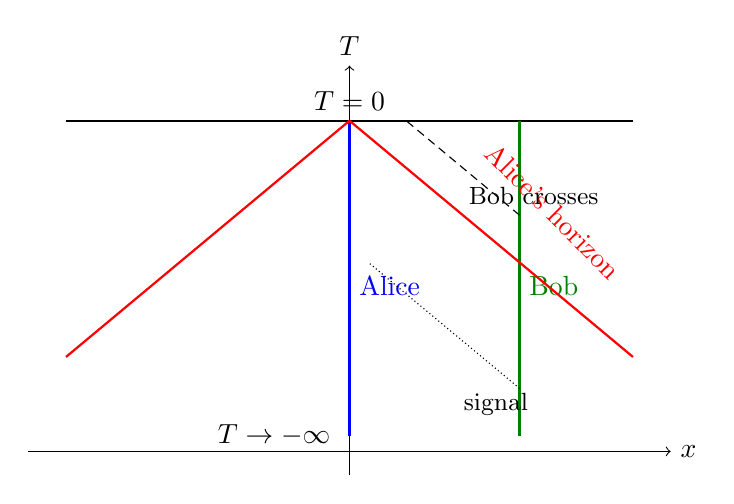
\begin{tikzpicture}[x=1.2cm,y=1.0cm]
\draw[thick] (-3,0) -- (3,0);
\node[above] at (0,0) {$T=0$};

\draw[->] (-3.4,-4.2) -- (3.4,-4.2) node[right] {$x$};
\draw[->] (0,-4.5) -- (0,0.7) node[above] {$T$};
\node[left] at (-0.1,-4.0) {$T\to -\infty$};

\draw[blue,thick] (0,-4) -- (0,0);
\node[blue,right] at (0,-2.1) {Alice};

\draw[green!50!black,thick] (1.8,-4) -- (1.8,0);
\node[green!50!black,right] at (1.8,-2.1) {Bob};

\draw[red,thick] (0,0) -- (3,-3);
\draw[red,thick] (0,0) -- (-3,-3);
\node[red,rotate=-45] at (2.15,-1.15) {Alice's horizon};

\draw[densely dashed] (1.8,-1.2) -- (0.6,0);
\node at (1.95,-0.95) {\small Bob crosses};

\draw[densely dotted] (1.8,-3.4) -- (0.2,-1.8);
\node at (1.55,-3.6) {\small signal};

\end{tikzpicture}
\caption{Cautious transcript-backed reconstruction of the de Sitter conformal diagram used in the lecture. The top edge \(T=0\) is the infinite future in proper time, light rays follow \(45^\circ\) lines, and Alice's past light cone never covers the whole spacetime.}
\end{figure}

This is where the lecture cashes in the opening promise about horizons. Alice may wait longer and longer, and the region she has seen may grow, but no amount of waiting lets her see the entire spacetime. That failure is not a practical limitation; it is a geometric fact. Bob may once have exchanged signals with Alice, yet once his worldline passes outside her horizon he can no longer send her a message. The lecture then sharpens the point further. Even in situations where one is tempted to say that Alice can still ``see'' Bob in some limiting sense, the signal is so extremely redshifted that it becomes physically useless. Causal loss and observational loss merge.

The lecture closes with one further geometric observation. The proper distance to the horizon stays fixed. In conformal coordinates the coordinate location of the horizon moves inward, but the conformal factor grows, and the two effects balance. This is the geometric version of the earlier statement that \(H\) remains constant and that the characteristic distance scale \(c/H\) does not change.

\section{Summary}

The lecture moves in a very definite sequence. Vacuum energy first appears as zero-point energy and virtual-fluctuation energy. Its crucial property is then isolated: unlike ordinary matter, it does not pick out a preferred Lorentz frame and does not dilute when space expands. Gravity makes that property physically consequential, because gravity couples to energy.

With the spatially flat expanding metric \(ds^2=-dt^2+a(t)^2dx^2\), the Friedmann equation reduces cosmology to an equation for \(a(t)\). Ordinary matter gives \(\rho_m\propto a^{-3}\), which leads to \(a(t)\propto t^{2/3}\) and a decelerating universe. Vacuum energy gives \(\rho_{\rm vac}=\text{const.}\), which leads to \(\dot a=Ha\) and therefore \(a(t)=Ce^{Ht}\), an accelerating universe. The observed universe appears to cross from the first behavior to the second.

Only after that cosmological spine is established does the lecture turn to horizons. The late-time vacuum-dominated spacetime is de Sitter space. By compressing the infinite future into the surface \(T=0\), one can draw its causal structure so that light rays run at \(45^\circ\). The result is the lecture's final point: every observer in de Sitter space has a private event horizon, and in the far future the universe becomes not merely dilute but causally lonely.